\section*{Running Program + Output}
To run the program all you need to do is double click the \textbf{\textit{icsParser}} executable.

\\
\begin{center}
   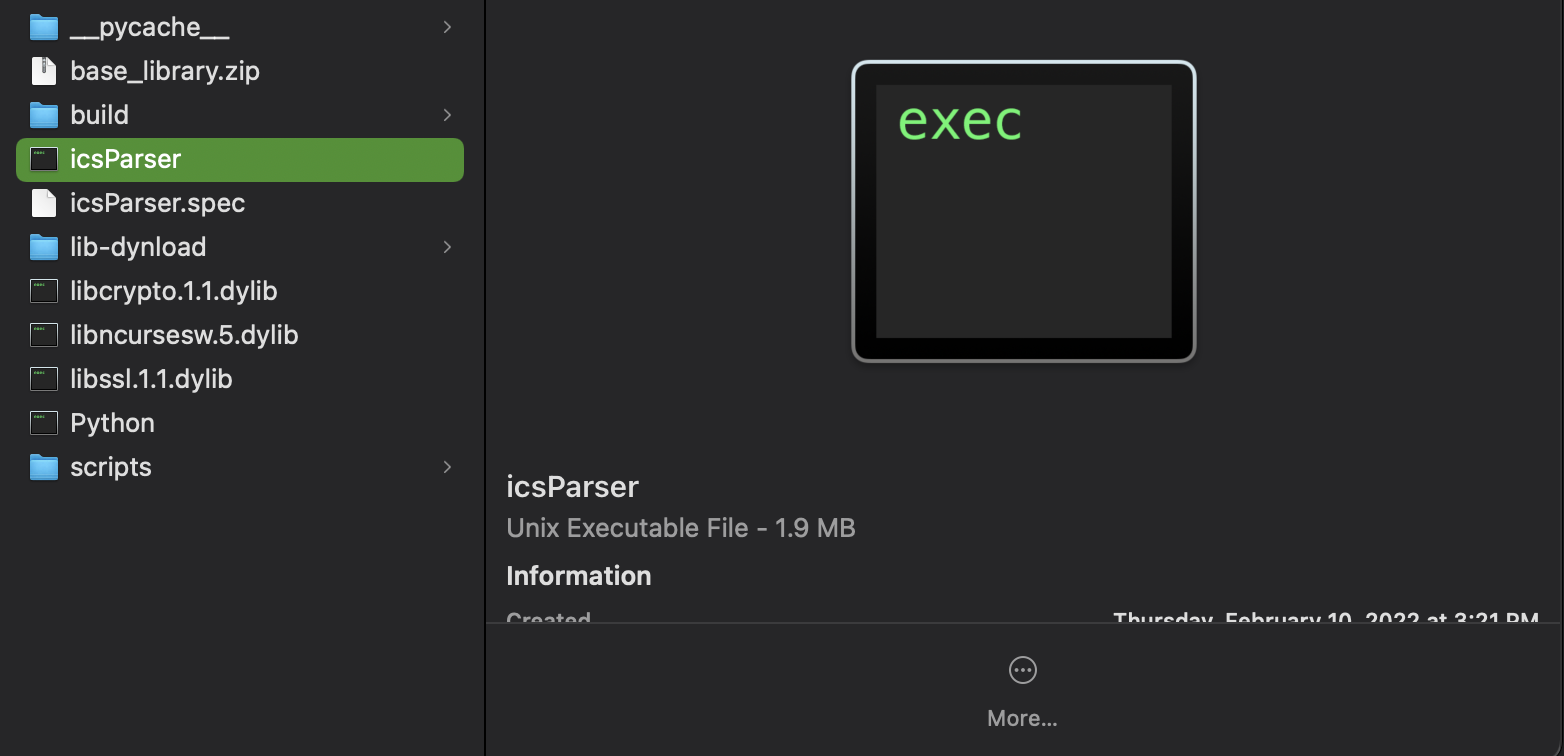
\includegraphics[width=100mm]{images/exe.png} 
\end{center}
\\
This will open up a terminal prompt that will tell you what files the program found if any and if the program ran successfully. You can ignore the I/O trace-back.
\\
\begin{center}
   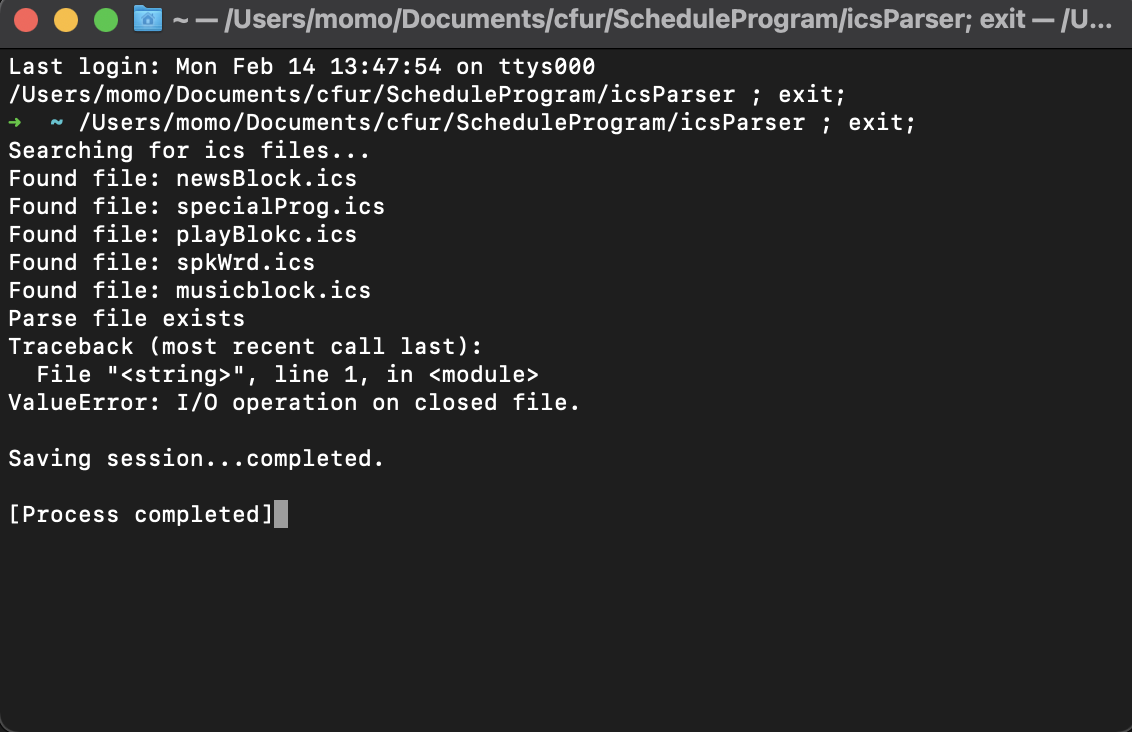
\includegraphics[width=100mm]{images/terminal.png}
\end{center}
\\
The output file can be found inside the \textbf{\textit{scripts}} folder along with the script file that will be used in Adobe Illustrator.
